%   DOCUMENT CLASS  %%%%%%%%%%%%%%%%%%%%%%%%%%%%%%%%%%%%%%%%%%%%%%%%%%%%%%%%%%%
%
%   Use the `sfuthesis` class to format your thesis. If your program does not
%   require a thesis defence, use the class option `undefended` like so:
%
%     \documentclass[undefended]{sfuthesis}
%
%   To generate a signature page for your defence, use the `sfuapproval` class
%   instead, by replacing the below line with
%
%     \documentclass{sfuapproval}
%
%   For more information about thesis formatting requirements, go to
%
%     http://www.lib.sfu.ca/help/publish/thesis
%
%   or ask a thesis advisor at the SFU Research Commons.
%

\documentclass{sfuthesis}



%   DOCUMENT METADATA  %%%%%%%%%%%%%%%%%%%%%%%%%%%%%%%%%%%%%%%%%%%%%%%%%%%%%%%%
%
%   Fill in the following information for the title page and approval page.
%

\title{Real-Time Neural Machine Translation}
\thesistype{Depth Report}
\author{Ashkan Alinejad}
\previousdegrees{%
	M.Sc., University of Tehran, 2016\\
	B.Sc., Shahid Beheshti University, 2014}
\degree{Doctor of Philosophy}
\discipline{Computer Science}
\department{Department of Computer Science}
\faculty{}
\copyrightyear{2017}
\semester{Fall 2017}
\date{January 10, 2017}

\keywords{Neural Machine Translation; Real-Time; SNMT}

\committee{%
	\chair{Pamela Isely}{Professor}
	\member{Emmett Brown}{Senior Supervisor\\Professor}
	\member{Bonnibel Bubblegum}{Supervisor\\Associate Professor}
	\member{James Moriarty}{Supervisor\\Adjunct Professor}
	\member{Kaylee Frye}{Internal Examiner\\Assistant Professor\\School of Engineering Science}
	\member{Hubert J.\ Farnsworth}{External Examiner\\Professor\\Department of Quantum Fields\\Mars University}
}



%   PACKAGES %%%%%%%%%%%%%%%%%%%%%%%%%%%%%%%%%%%%%%%%%%%%%%%%%%%%%%%%%%%%%%%%%%
%
%   Add any packages you need for your thesis here.
%   You don't need to call the following packages, which are already called in
%   the sfuthesis class file:
%
%   - appendix
%   - etoolbox
%   - fontenc
%   - geometry
%   - lmodern
%   - nowidow
%   - setspace
%   - tocloft
%
%   If you call one of the above packages (or one of their dependencies) with
%   options, you may get a "Option clash" LaTeX error. If you get this error,
%   you can fix it by removing your copy of \usepackage and passing the options
%   you need by adding
%
%       \PassOptionsToPackage{<options>}{<package>}
%
%   before \documentclass{sfuthesis}.
%
%   The following packages are a few suggestions you might find useful.
%
%   (1) amsmath and amssymb are essential if you have math in your thesis;
%       they provide useful commands like ``blackboard bold'' symbols and
%       environments for aligning equations.
%   (2) amsthm includes allows you to easily change the style and numbering of
%       theorems. It also provides an environment for proofs.
%   (3) graphicx allows you to add images with \includegraphics{filename}.
%   (4) hyperref turns your citations and cross-references into clickable
%       links, and adds metadata to the compiled PDF.
%   (5) pdfpages lets you import pages of external PDFs using the command
%       \includepdf{filename}. You will need to do this if your research
%       requires an Ethics Statement.
%

\usepackage{amsmath}                            % (1)
\usepackage{amssymb}                            % (1)
\usepackage{amsthm}                             % (2)
\usepackage{graphicx}                           % (3)
\usepackage{caption}
\usepackage[pdfborder={0 0 0}]{hyperref}        % (4)
% \usepackage{pdfpages}                         % (5)
% ...
% ...
% ...
% ... add your own packages here!




%   OTHER CUSTOMIZATIONS %%%%%%%%%%%%%%%%%%%%%%%%%%%%%%%%%%%%%%%%%%%%%%%%%%%%%%
%
%   Add any packages you need for your thesis here. We've started you off with
%   a few suggestions.
%
%   (1) Use a single word space between sentences. If you disable this, you
%       will have to manually control spacing around abbreviations.
%   (2) Correct the capitalization of "Chapter" and "Section" if you use the
%       \autoref macro from the `hyperref` package.
%   (3) The LaTeX thesis template defaults to one-and-a-half line spacing. If
%       your supervisor prefers double-spacing, you can redefine the
%       \defaultspacing command.
%

\frenchspacing                                    % (1)
\renewcommand*{\chapterautorefname}{Chapter}      % (2)
\renewcommand*{\sectionautorefname}{Section}      % (2)
\renewcommand*{\subsectionautorefname}{Section}   % (2)
% \renewcommand{\defaultspacing}{\doublespacing}  % (3)
% ...
% ...
% ...
% ... add your own customizations here!


\setlength\abovecaptionskip{-10pt}

%   FRONTMATTER  %%%%%%%%%%%%%%%%%%%%%%%%%%%%%%%%%%%%%%%%%%%%%%%%%%%%%%%%%%%%%%
%
%   Title page, committee page, copyright declaration, abstract,
%   dedication, acknowledgements, table of contents, etc.
%
%   If your research requires an Ethics Statement, download one from the
%   SFU library website and uncomment the appropriate lines below.
%

\begin{document}

\frontmatter
\maketitle{}
%\makecommittee{}

%\addtoToC{Ethics Statement}%
%\includepdf[pagecommand={\thispagestyle{plain}}]{ethicsstatement.pdf}%
%\clearpage

\begin{abstract}
	Studies on Machine Translation (MT) has a long history, but most of the works in this area assumes we can have access to the entire sentences. As a result, it is not practical to apply them on Real-Time Machine Translation where the objective is to start translation \textit{before} receiving the full sentences. Divergent syntax of different languages makes it a great challenge for both humans and machines to start translating while new inputs are still being received.\\
	Over the past few years, the great success of using deep neural networks in Real-Time translation systems, led this field to evolve in completely new direction and improved the results; However, many of the problems from conventional systems remained unsolved. This report provides a review over the latest methods of utilizing neural attention models for the task of simultaneous machine translation.
	
\end{abstract}


%\begin{dedication}
%	This is an optional page.
%\end{dedication}


%\begin{acknowledgements}
%	This is an optional page.
%\end{acknowledgements}

\addtoToC{Table of Contents}%
\tableofcontents%
\clearpage

\addtoToC{List of Tables}%
\listoftables%
\clearpage

\addtoToC{List of Figures}%
\listoffigures%
\clearpage





%   MAIN MATTER  %%%%%%%%%%%%%%%%%%%%%%%%%%%%%%%%%%%%%%%%%%%%%%%%%%%%%%%%%%%%%%
%
%   Start writing your thesis --- or start \include ing chapters --- here.
%

\mainmatter%

%++++++++++++++++++++++++++++++++++++++++++++++++++++++++++++++++++++++++++
\chapter{Introduction}

\section{Recurrent Neural Networks} \label{sec:RNN}

\subsection{Long Short-Term Memory}

\subsection{Gated Recurrent Units}

\section{Evaluation Methods}
\subsection{BLEU Score}
\subsection{ROUGE Score}

%++++++++++++++++++++++++++++++++++++++++++++++++++++++++++++++++++++++++++
\chapter{Traditional Systems}



%++++++++++++++++++++++++++++++++++++++++++++++++++++++++++++++++++++++++++
\chapter{Neural Machine Translation}
Neural Networks can be seen as an essential component in most of recent approaches in the field of machine translation. In section \ref{sec:RNN} we have reviewed various components of RNNs\footnote{Recurrent Neural Networks} . During this chapter, we will describe how we can use them to build translation systems that can extract semantic information from source language and follow the syntactical structure of target language in order to produce translated words.

\section{Neural Translation Models} \label{sec:NTM}
Most of the state-of-the-art approaches toward solving Machine Translation uses the Encoder-Decoder architecture with attention; However, since adding attention mechanism makes the structure more complex, we will start with simple Encoder-Decoder translation systems in the next section. Later, in \ref{sub:attention} we will demonstrate how attention mechanism affects the translation process.
\subsection{Encoder-Decoder structure} \label{sub:EncDec}
The very basic neural structure that can generate reasonable translations is what is called the \textbf{Encoder-Decoder} model \cite{Chrisman:1991:EncDec, Sutskever:2014:NIPS}. The concept of this model is to use stacked layers of LSTM cells in order to \emph{encode} the whole source sentence into a real-valued vector. Then we can feed this vector to our second neural network to \emph{decode} it and produce translated words one at a time. see figure \ref{fig:EncDec0} for illustration.\\
More mathematically, our network at time step $t$ will receive a numerical representation of word $x_t$ from the source sentence $X = [x_1, \dots, x_T]$. Then it will combine them with output of encoder at previous time step and passes them to a non-linear function. In other words: $h_t = f(x_t, h_{t-1})$, where $f$ is a non-linear function. Once the encoder receives the <eos> word, it will start to compute the final encoder's context vector $h_T$.\\
In decoder component, we will use the output from previous time step $y_{i-1}$, previous decoder output $s_{i-1}$ as well as $h_T$, as an input for decoder's neural network. We will compute $s_{i}$, similar to encoder's context vector, with $s_{i} = g(y_{i-1}, s_{i-1}, h_{T})$, where $g$ is a non-linear function. Then we will pass $s_i$ through a softmax layer in order to compute the probability $P(y_i | X, y_{<i})$.  We will choose $y_i$ that maximizes the probability. i.e. $i = \arg\max_{y_i} P(y_i | X, y_{<i}$).\\
This is the very basic, yet powerful structure of the encoder-decoder model and while there are lots of neural models for machine translation, these can be seen as extensions to this model. In \cite{Sutskever:2014:NIPS} it is shown that with some refinements (E.g. using BiLSTM instead of LSTM as encoder), the encoder-decoder structure can beat most of the approaches with many years of research in their background. We will talk about these techniques in the next two sections.
\begin{figure}[t]
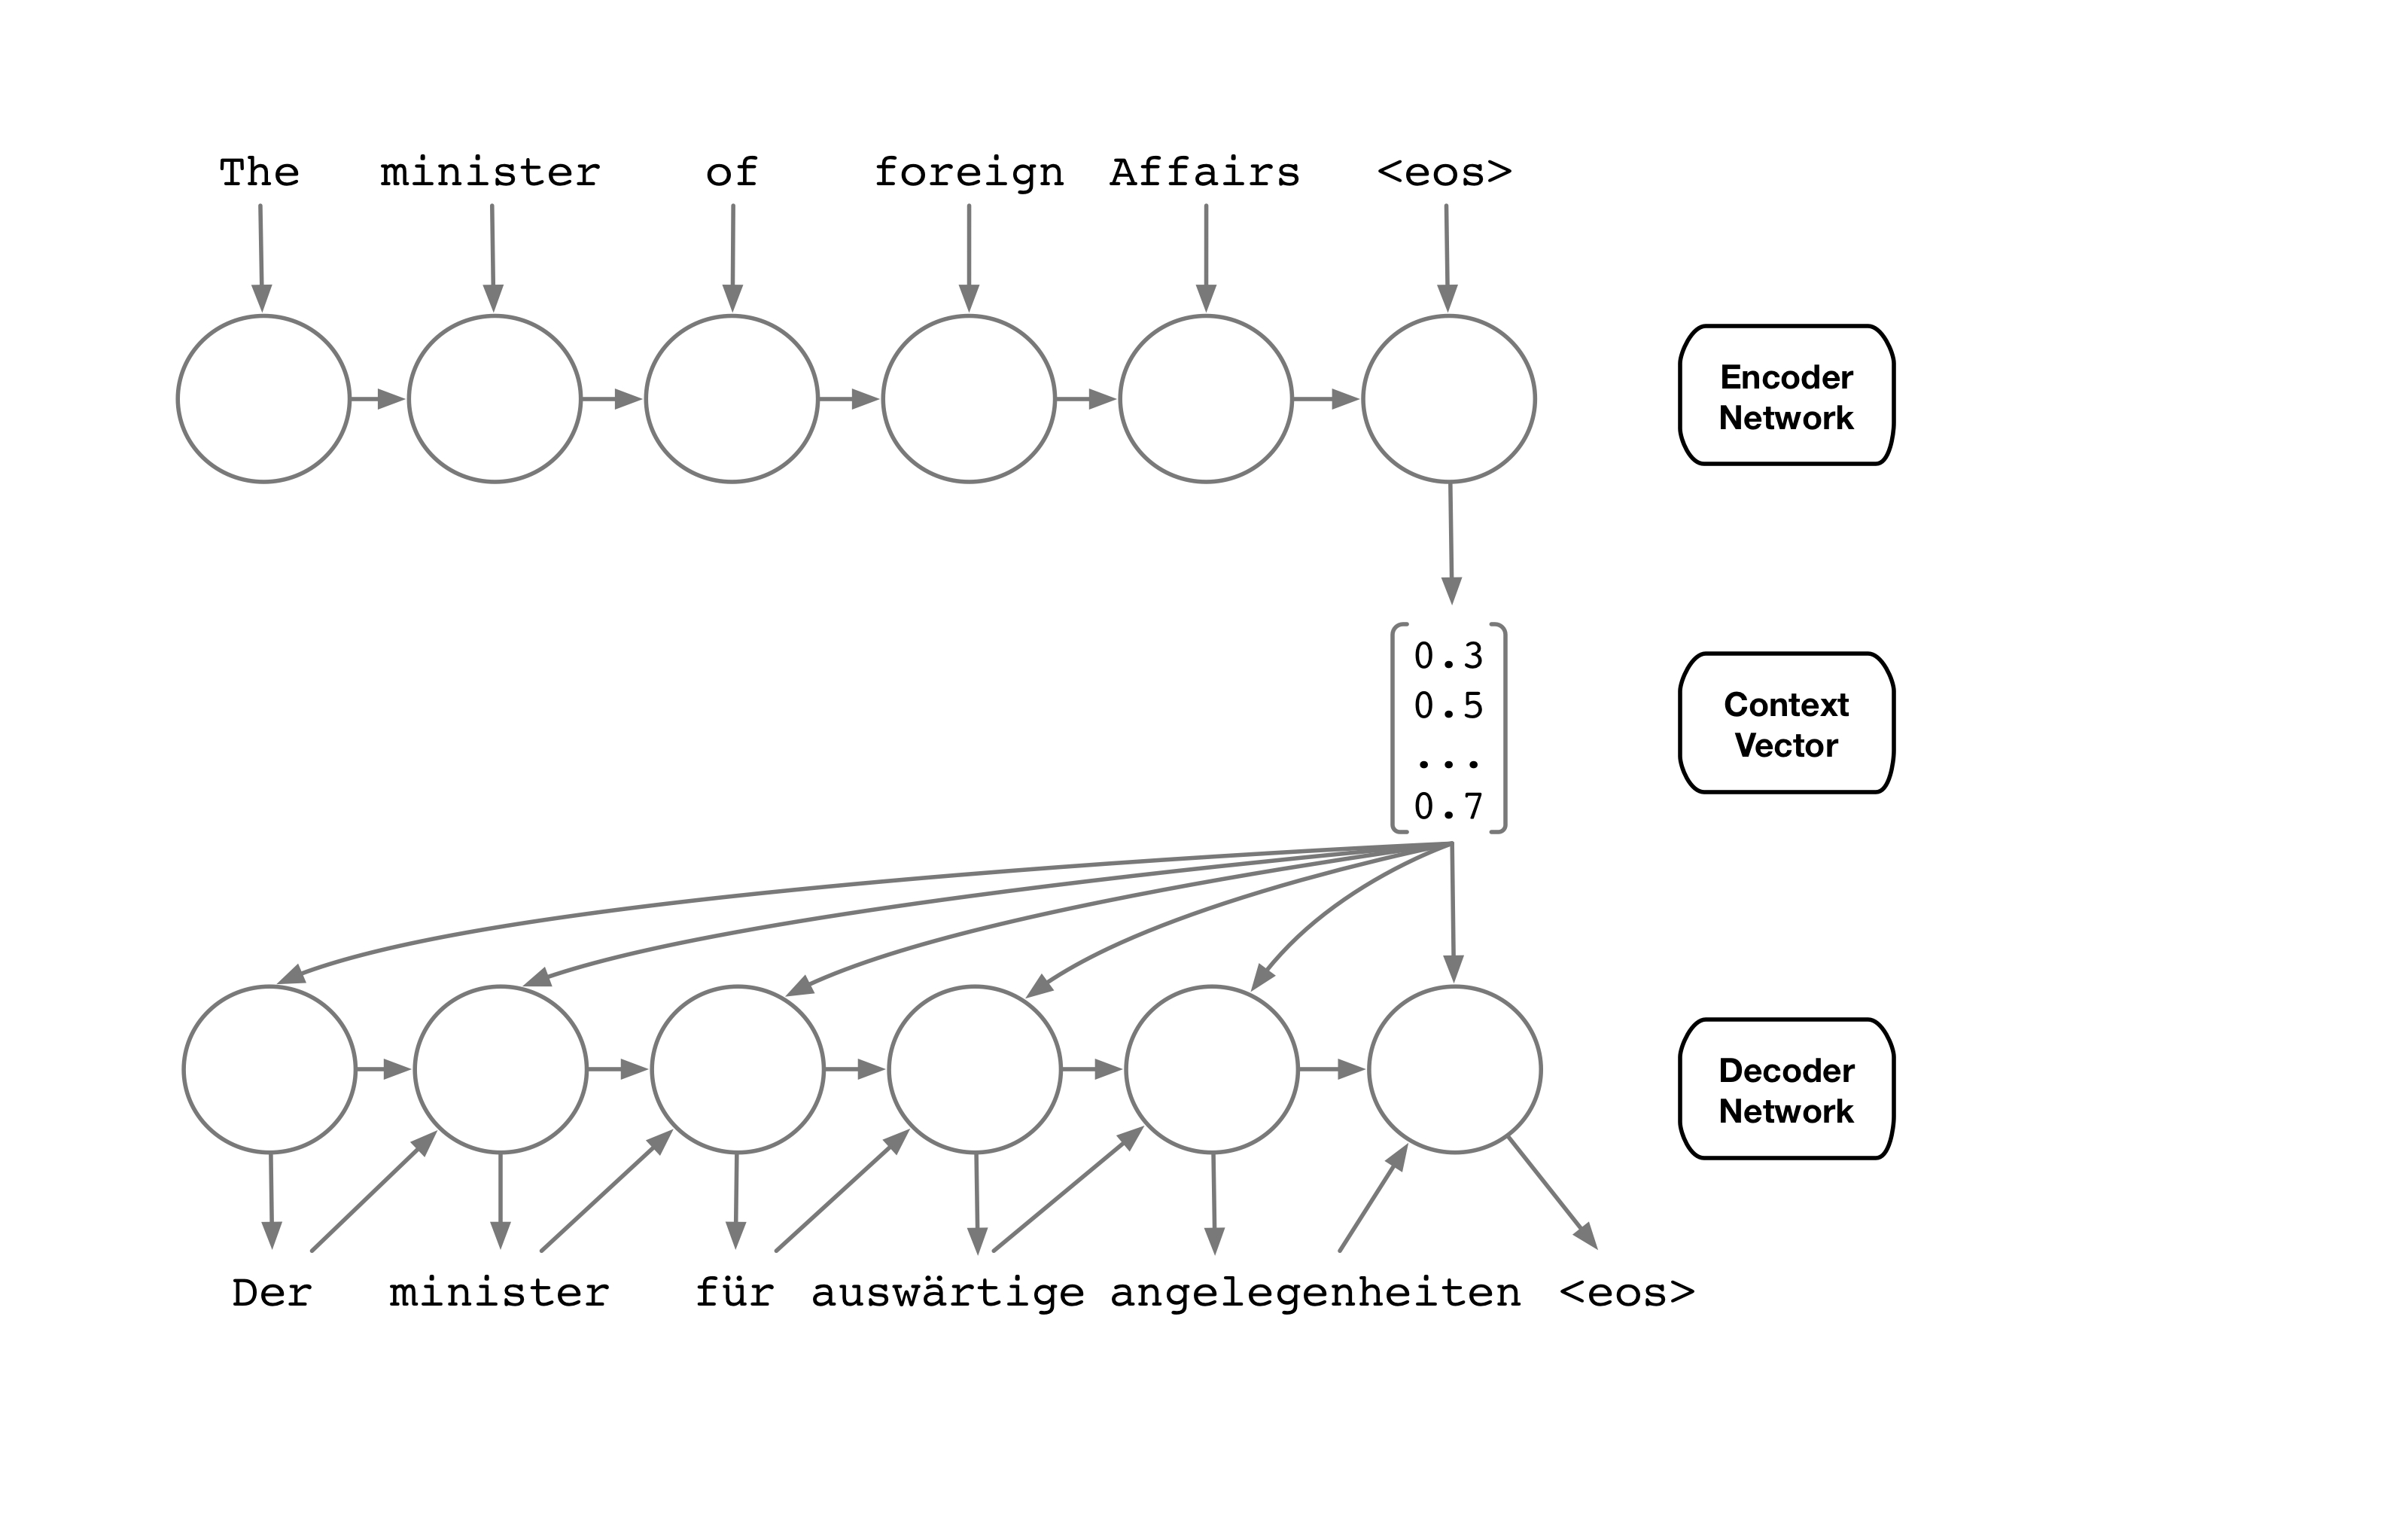
\includegraphics[scale=0.15]{./images/EncDec0}
\caption{Structure of an Encoder-Decoder model.}
\label{fig:EncDec0}
\end{figure}

\subsection{Beam Search}

\subsection{Attention Mechanism} \label{sub:attention}
We are only one step away to look at the state-of-the-art translation model which is the encoder-decoder model with attention mechanism. As we have seen in \ref{sub:EncDec}, the encoder-decoder networks forces the encoder to keep all the information required for decoding into a fixed-dimensional context vector. On the other side of this structure, the decoder only have access to this context vector and it is supposed to produce the whole translation using this fixed representation of input.\\
Although, with keeping these restrictions in mind, the architecture works well, as the length of sentences grows, the decoder's performance decreases a lot. In order to fix these constraints, Bahdanau et al. \cite{Bahdanau:2014:Attention} proposes the attention mechanism. The main idea is that instead of using the last state of the encoder's context vector, the decoder is able to use a weighted combination of encoder's output at different time steps. As a result, Not only the decoder would be powerful, but it would also be much more easier for encoder to encode input sentences at each time step. \\
More concretely, the first component of this structure encodes the embeddings of input words $X=\{ x_1, \dots, x_{T_s} \}$ into context vectors $H = \{ h_1, \dots, h_{T_s} \}$. It can be done by utilizing a bidirectional RNN:

$$h_i = \phi_{\text{BiRNN}}(h_{i-1}, x_i)$$
On decoder side we will have:
\begin{align}
\centering
&\alpha_i^\tau = \phi_{\text{ATTN}}(z_{\tau -1}, h_i)  \label{eq:att1} \\[1em]
&c_\tau = \sum_{i=1}^{T_x} \alpha_i^\tau h_i  \label{eq:att2} \\[1em]
&z_\tau = \phi_{\text{DEC}}(z_{\tau -1}, y_{\tau -1}, c_\tau)  \label{eq:att3} \\[1em]
&p(y|y_{<\tau}, H) \propto \text{exp} [\phi_{out} (z_{\tau}) ]  \label{eq:att4} \\[1em]
&y_{\tau} = \arg \max_y p(y|y_{<\tau}, H)
\end{align}
In equation \ref{eq:att1}, $z_{\tau - 1}$ is the decoder's context vector at previous time step and $\phi_{\text{ATTN}}$ is the attention function which can be any function that measures how well input at position $i$ is related to output at time step $\tau$. The most commonly used function is the original formula presented by Bahdanau et al \cite{Bahdanau:2014:Attention} which employs a multilayer feedforward neural network. We then pass these scores to a Softmax function in order to make their summation equal to one. The output of attention layer in equation \ref{eq:att2} is using $\alpha_i^\tau$ as probability as a means to compute a weighted average over the encoder's context vector.


\begin{figure}[t]
\centering
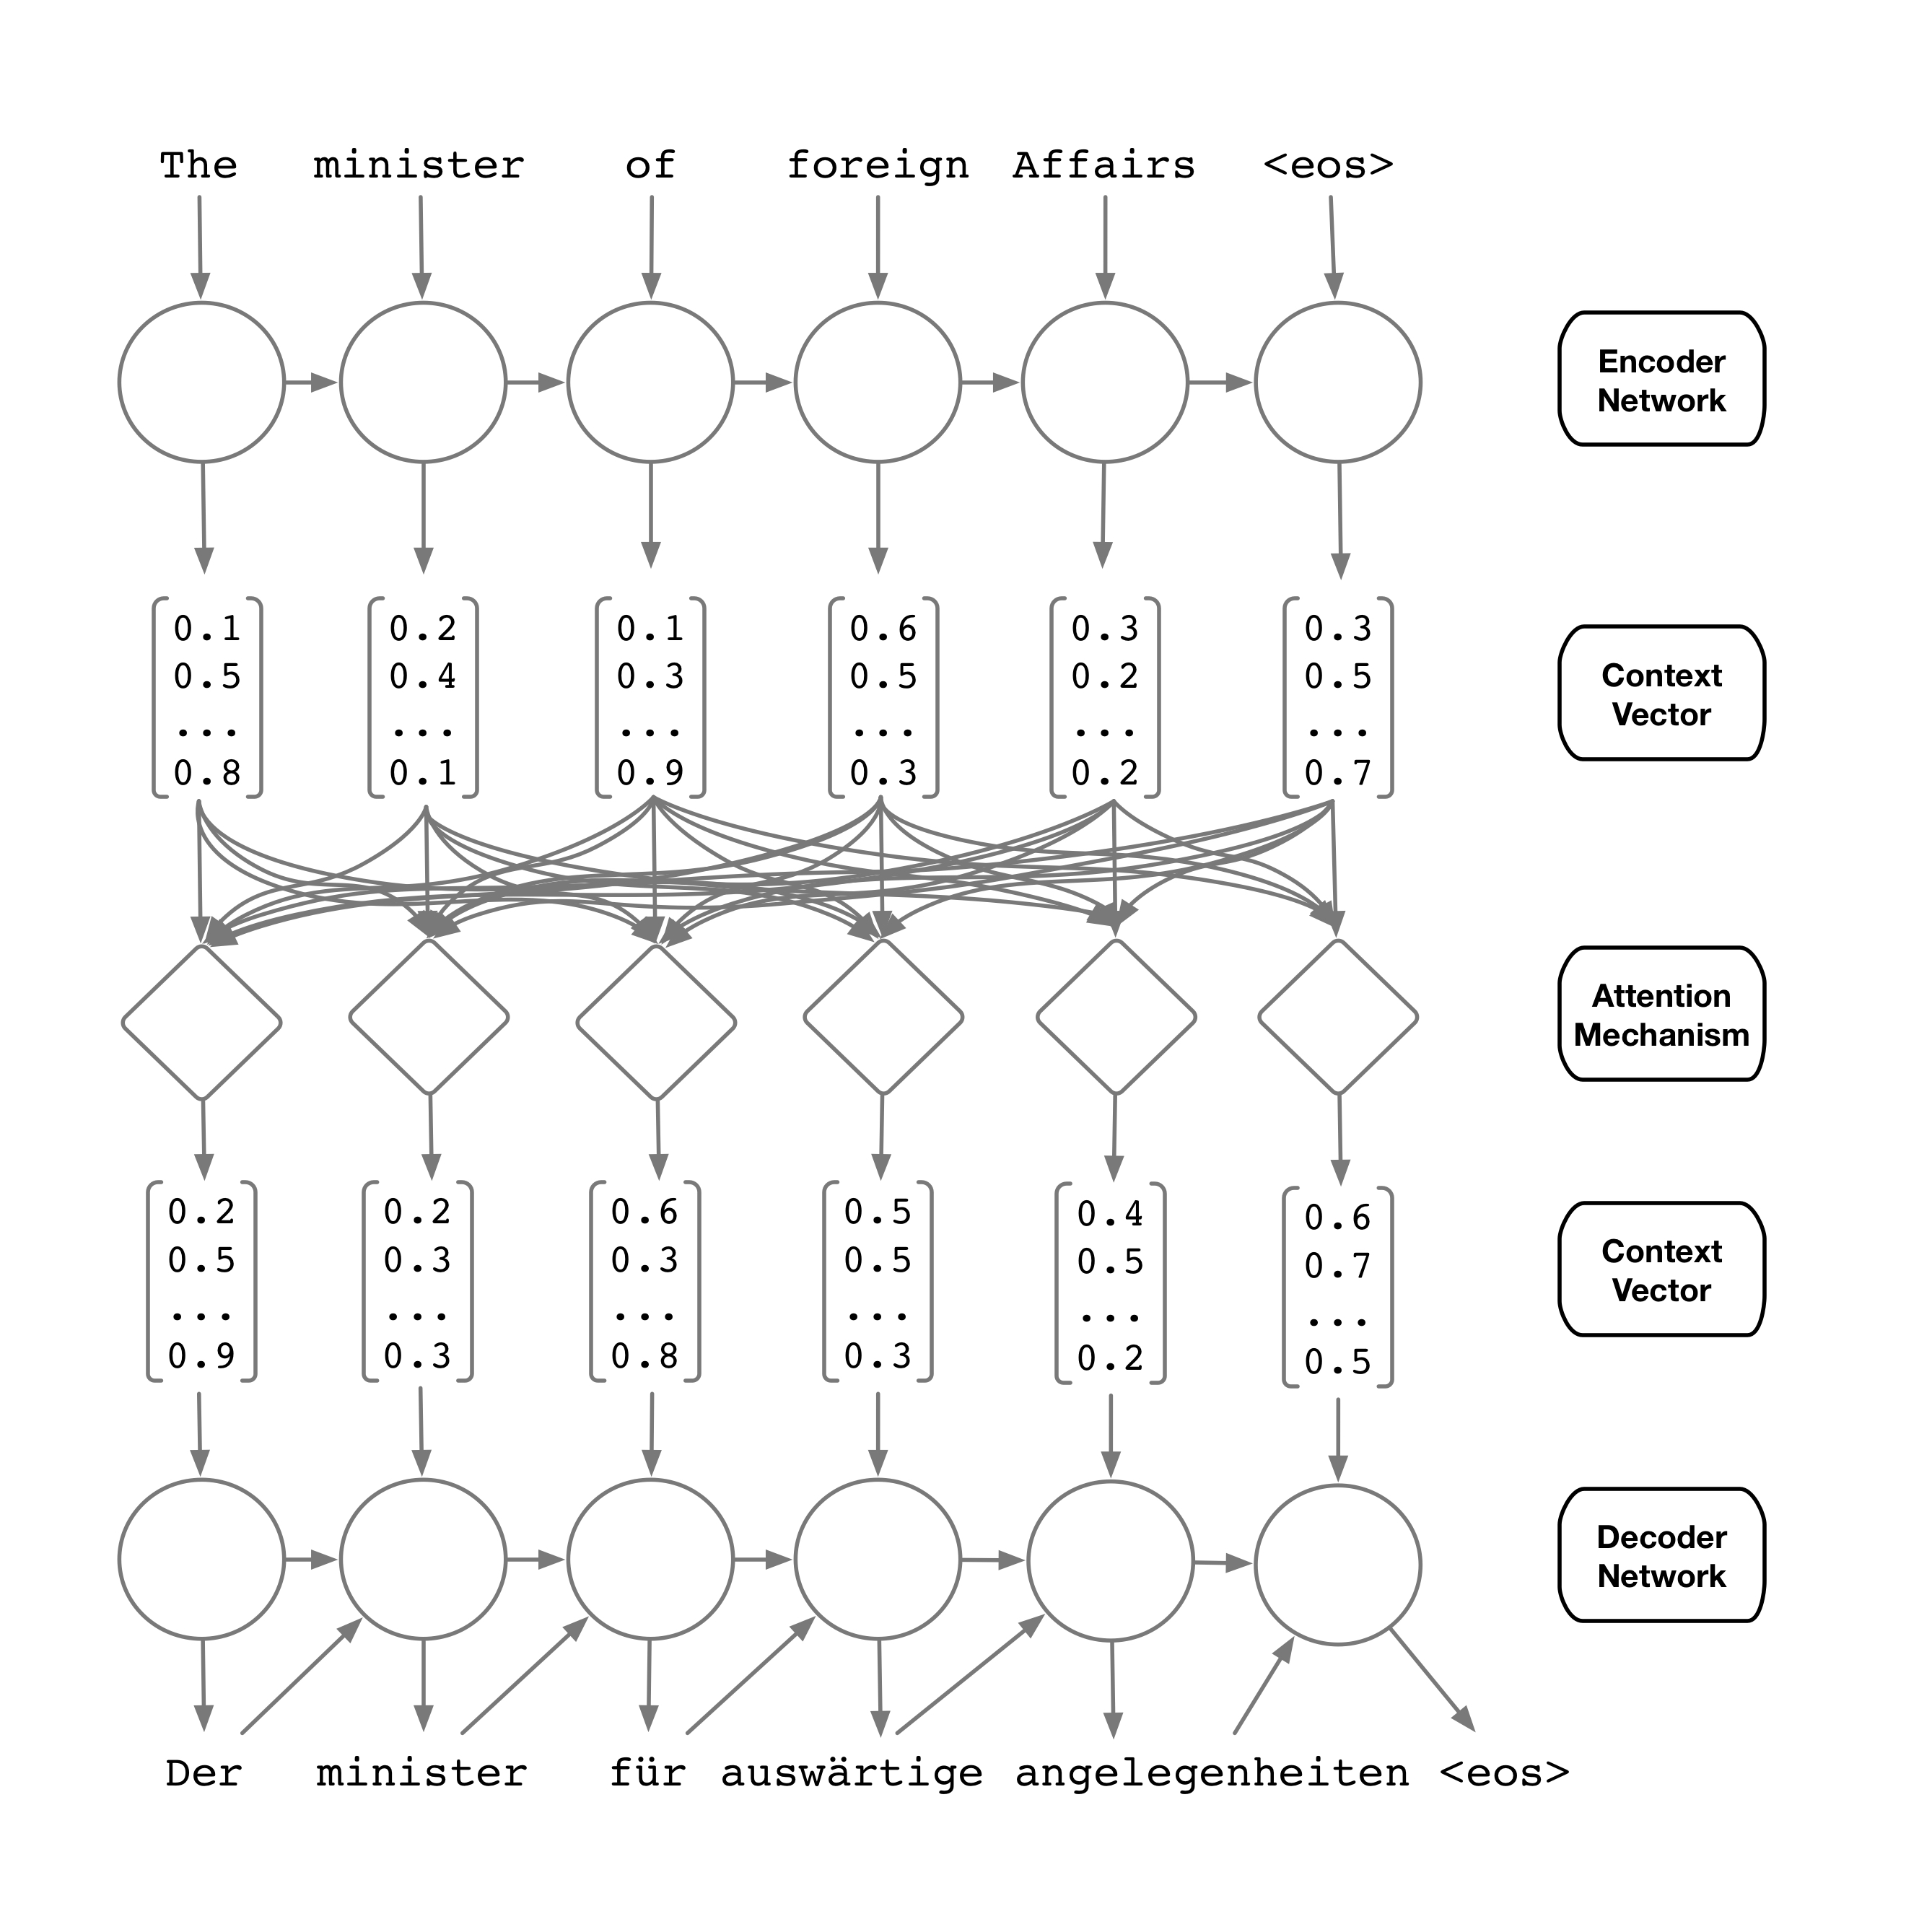
\includegraphics[scale=0.15]{./images/attention}
\caption{Structure of an Encoder-Decoder model with Attention mechanism.}
\label{fig:EncDec0}
\end{figure}


%++++++++++++++++++++++++++++++++++++++++++++++++++++++++++++++++++++++++++
\chapter{Real-Time Neural Machine Translation}
In the first section of this chapter we will talk about a new approach to solve the task of translation in real-time, presented by Cho et al. We will look at a novel decoding algorithm, called \textit{Simultaneous greedy decoding} which serves as the starting point of  new family of algorithms to allow neural translation systems begin translating before receiving the full sentence. Then we will describe another method based on simultaneous greedy decoding in section \ref{sec:TA}, which shows us how we can train our systems to learn when to segment a sentence based on predefined quality and delay criteria.

\section{Simultaneous Greedy Decoding} \label{sec:SGD}


\section{Learning Policy with Trainable Agent} \label{sec:TA}


%++++++++++++++++++++++++++++++++++++++++++++++++++++++++++++++++++++++++++
\chapter{Results and Analysis}


%++++++++++++++++++++++++++++++++++++++++++++++++++++++++++++++++++++++++++
\chapter{Conclusion}



%   BACK MATTER  %%%%%%%%%%%%%%%%%%%%%%%%%%%%%%%%%%%%%%%%%%%%%%%%%%%%%%%%%%%%%%
%
%   References and appendices. Appendices come after the bibliography and
%   should be in the order that they are referred to in the text.
%
%   If you include figures, etc. in an appendix, be sure to use
%
%       \caption[]{...}
%
%   to make sure they are not listed in the List of Figures.
%

\backmatter%
	\addtoToC{Bibliography}
	\bibliographystyle{plain}
	\bibliography{references}

%\begin{appendices} % optional
%	\chapter{Code}
%\end{appendices}
\end{document}
